
\section{Variables aleatorias discretas}

Supongamos que a cada punto del espacio muestral se le asigna un número.  Entonces hemos definido una \emph{función} en el espacio muestral  Esta función es llamada \emph{variable aleatoria} (o \emph{variable estocástica}) o de manera más precisa \emph{función aleatoria}. 


Usualmente, las variables aleatorias se denotan por letras mayúsculas como $X$ o $Y$. En general, una variable aleatoria tiene algún significado físico, geométrico, económico, financieros, etc.



\begin{ejemplo}
	\label{exmp:2.1}
	Supongamos que una moneda se lanza dos veces de manera que el espacio muestral es $\set{HH,HT,TH,TT}.$  Digamos que $X$ representa el número de soles ($H$) que obtenemos.
\end{ejemplo}


\subsection{Funciones de probabilidad discretas}

Sea $X$ una variable aleatoria discreta.  Supongamos que los valores que puede tomar son $x_{1},...,x_{k},$ arreglados en algún orden dado.  Supongamos también que esos valores
tienen alguna probabilidad dada por
\begin{align}
	\label{2.1}
	P(X=x_{k})=f(x_{k}).
\end{align}


{Función de probabilidad}
\begin{align}
	\label{2.2}
	P(X=x)=
	\begin{cases}
		f(x) & x=x_{k} \\
		0	& \text{en otro caso}
	\end{cases}
\end{align}



En general, $f(x)$ será una función de probabilidad si
\begin{align}
	\begin{cases}
		f(x)\geq 0 \\
		\sum_{x}f(x)=1.
	\end{cases}
\end{align}



\begin{ejemplo}
	\label{exmp:2.2}
	Encuentre la función de probabilidad correspondiente a la variable aleatoria $X$ del ejemplo \ref{exmp:2.1}.
\end{ejemplo}



\begin{ejemplo}
	\label{sol:2.1}
	Suponga que un par de dados se lanzan. Sea $X$ la variable aleatoria dada por la suma de los puntos. Encuentre la distribución de probabilidad de $X.$
\end{ejemplo}



\begin{ejemplo}
	\label{sol:2.2}
	Encuentre la distribución de probabilidad de niños y niñas en familias con 3 hijos, suponiendo la misma probabilidad para niños y niñas.
\end{ejemplo}



\subsection{Funciones de distribución para variables aleatorias discretas}


La función de distribución de una variable discreta $X$ se obtiene de la función de probabilidad a través de la siguiente fórmula
\begin{align}
	\label{2.4}
	F(x) = P(X\leq x) = \sum_{u \leq x} f(u).
\end{align}



Si $X$ toma sólo un número finito de valores $x_{1},...,x_{n}$ entonces la función de distribución está dada por
\begin{align}
	\label{2.5}
	F(x)=
	\begin{cases}
		0 & -\infty < x < 0 \\
		f(x_{1}) & x_{1} \leq x < x_{2} \\
		f(x_{1})+f(x_{2}) & x_{2} \leq x < x_{3} \\
		\vdots & \vdots \\
		f(x_{1})+\cdots+f(x_{n}) & x_{n} \leq x < \infty
	\end{cases}
\end{align}



\begin{ejemplo}
	\label{exmp:2.3}
	Encuentre la función de distribución para la variable aleatoria $X$ del ejemplo \ref{exmp:2.2} y obtenga su gráfica.
\end{ejemplo}



\begin{figure}
	\centering
	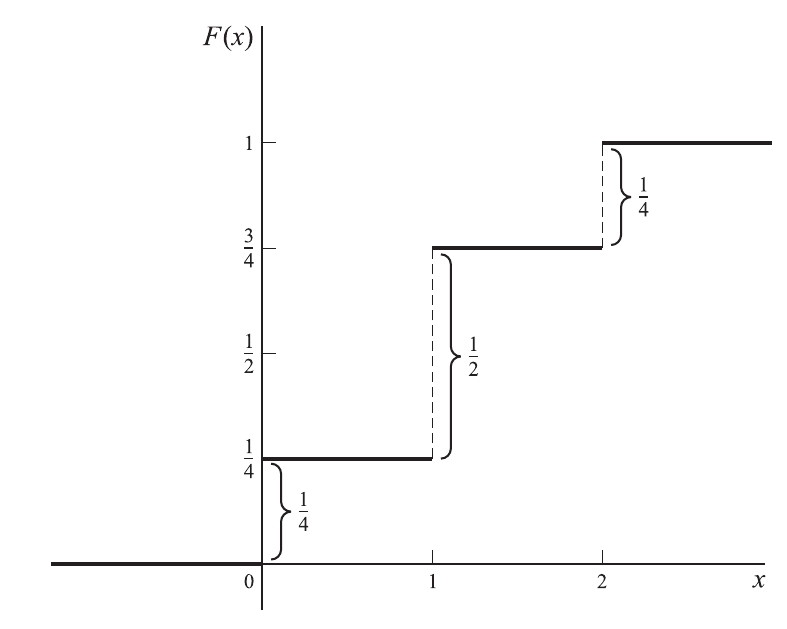
\includegraphics[height=7cm,keepaspectratio=true]{./pe/pands0201.png}
	% pands0201.png: 0x0 pixel, 300dpi, 0.00x0.00 cm, bb=
	\label{fig:0201}
\end{figure}



\begin{observacion}
	\begin{itemize}
		\item Los saltos en la función de distribución están determinados por el valor de la función de probabilidad. 
		\item Este tipo de funciones se conoce como \emph{función escalonada}.  Debe observarse que son \emph{continuas por la derecha.}
		\item La función de distribución es \emph{monótonamente creciente.}
	\end{itemize}
	
\end{observacion}



La función de probabilidad se puede obtener a partir de la función de distribución con la siguiente fórmula
\begin{align}
	\label{2.6}
	f(x)=F(x)-\lim_{u \to x^{-}}F(u).
\end{align}



\begin{ejemplo}
	\label{sol:2.3}
	\begin{enumerate}
		\item Encuentre la función de distribución $F(x)$ para la variable aleatoria del problema resuelto \ref{sol:2.1};
		\item grafique esta función de distribución.
	\end{enumerate}
	
\end{ejemplo}



\begin{figure}
	\centering
	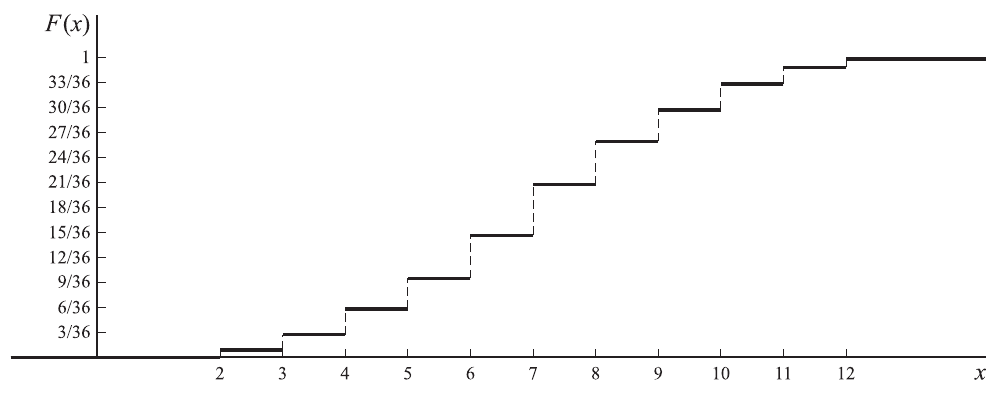
\includegraphics[width=10cm,keepaspectratio=true]{./pe/pands0206.png}
	% pands0206.png: 0x0 pixel, 300dpi, 0.00x0.00 cm, bb=
\end{figure}




\begin{ejemplo}
	\label{sol:2.4}
	\begin{enumerate}
		\item Encuentre la función de distribución $F(x)$ para la variable aleatoria del problema resuelto \ref{sol:2.2};
		\item grafique esta función de distribución.
	\end{enumerate}
	
\end{ejemplo}



\begin{figure}
	\centering
	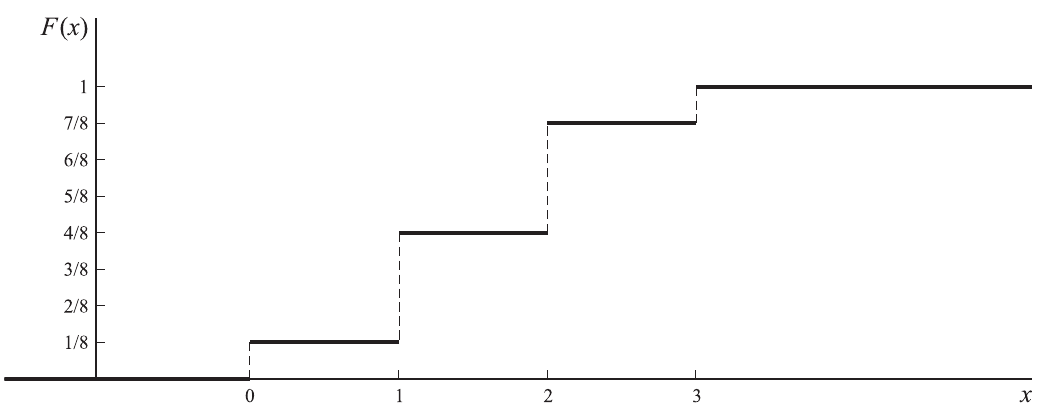
\includegraphics[width=10cm,keepaspectratio=true]{./pe/pands0207.png}
	% pands0206.png: 0x0 pixel, 300dpi, 0.00x0.00 cm, bb=
\end{figure}

